\documentclass[british,a4paper,order=firstname]{mathscript}
\usepackage{mathoperators}

\title{\textbf{Applied statistics: Coursework 1}}
\author{\person{Henry Haustein}}

\begin{document}
\pagenumbering{roman}
\pagestyle{plain}

\maketitle

\hypertarget{tocpage}{}
\tableofcontents
\bookmark[dest=tocpage,level=1]{Table of contents}

\pagebreak
\pagenumbering{arabic}
\pagestyle{fancy}

\section{Task 1}
\subsection{Part (1)}
In the given data were two out of 26 data points with an Al/Be ratio of more than 4.5. That means
\begin{align}
	\hat{p} = \frac{2}{26} = \frac{1}{13}\notag
\end{align}

\subsection{Part (2)}
Using the following formula from the lecture we get the 95\% confidence interval:
\begin{align}
	\hat{p}&\pm 2\cdot\sqrt{\frac{\hat{p}(1-\hat{p})}{n}} \notag \\
	\frac{1}{13} &\pm \underbrace{2\cdot\sqrt{\frac{\frac{1}{13}\cdot\frac{12}{13}}{26}}}_{0.1045} \notag
\end{align}
Our 95\% confidence interval is [-0.0276,0.1814] which means that we are 95\% sure that the true proportion lies between -0.0276 and 0.1814. 

\subsection{Part (3)}

\subsection{Part (4)}

\pagebreak
\section{Task 2}
\subsection{Part (1)}
\begin{lstlisting}
x = [-4.5, -1, -0.5, -0.15, 0, 0.01, 0.02, 0.05, ...
0.15, 0.2, 0.5, 0.5, 1, 2, 3];
m = mean(x);
s = std(x);
\end{lstlisting}
\begin{center}
	\begin{tabular}{p{4cm}|p{7cm}}
		null hypothesis & $H_0$: $\mu = 0$ \\
		\hline
		alternative hypothesis & $H_A$: $\mu\neq 0$ \\
		\hline
		t-test for $\mu$ & $t=\frac{m-0}{\frac{s}{\sqrt{15}}} =\frac{0.0853}{\frac{1.6031}{\sqrt{15}}} = 0.2062$ \\
		\hline
		rejection region & \texttt{tinv(0.05,15)} = -1.7531 \\
		\hline
		conclusion & $t$ is not in the rejection region so $H_0$ is accepted at the 10\% significance level.
	\end{tabular}
\end{center}
\begin{center}
	\begin{tikzpicture}
	\begin{axis}[
	xmin=-3, xmax=3, xlabel=$x$,
	ymin=0, ymax=1, ylabel=$y$,
	samples=400,
	axis y line=middle,
	axis x line=middle,
	domain=-3:3,
	restrict y to domain=0:1,
	width = 16cm,
	height = 8cm,
	]
	\addplot[name path=f,blue] {116640000000*sqrt(15)/(143*pi*(x^2+15)^(8))};
	\path[name path=axis] (axis cs:1.7531,0) -- (axis cs:3,0);
	\path[name path=axis2] (axis cs:-3,0) -- (axis cs:-1.7531,0);
	\draw (axis cs:1.7531,0) -- (axis cs:1.7531,1);
	\draw (axis cs:-1.7531,0) -- (axis cs:-1.7531,1);
	\draw [dotted] (axis cs:0.2062,0) -- (axis cs:0.2062,0.6);
	\node at (axis cs:1,0.5) (a) {0.05};
	\node at (axis cs:-1,0.5) (a2) {0.05};
	\draw (axis cs:1, 0.46) -- (axis cs: 2.2,0.02);
	\draw (axis cs:-1, 0.46) -- (axis cs: -2.2,0.02);
	\node at (axis cs: 2.0,0.95) (b) {1.7531};
	\node at (axis cs: -2.0,0.95) (b2) {-1.7531};
	\node at (axis cs: 0.45,0.55) (c) {0.2062};
	\node[red] at (axis cs: 2.4,0.78) (d) {rejection region};
	\node[red] at (axis cs: -2.4,0.78) (d2) {rejection region};
	\begin{scope}[transparency group]
	\begin{scope}[blend mode=multiply]
	\addplot [thick,color=blue,fill=blue,fill opacity=0.3] fill between[of=f and axis,soft clip={domain=1.7531:3},];
	\addplot [thick,color=blue,fill=blue,fill opacity=0.3] fill between[of=f and axis2,soft clip={domain=-3:-1.7531},];
	\draw[red,fill=red,opacity=0.2] (axis cs: 1.7531,0) -- (axis cs: 1.7531,1) -- (axis cs: 3,1) -- (axis cs: 3,0) -- (axis cs: 1.7531,0);
	\draw[red,fill=red,opacity=0.2] (axis cs: -1.7531,0) -- (axis cs: -1.7531,1) -- (axis cs: -3,1) -- (axis cs: -3,0) -- (axis cs: -1.7531,0);
	\end{scope}
	\end{scope}
	\end{axis}
	\end{tikzpicture}
\end{center}

\subsection{Part (2)}
If we reduce the significance level our rejection region gets smaller. With $\alpha = 0.05$ the rejection region will start at \texttt{tinv(0.025,15)} = -2.1314. The $t$ calculated in part (1) won't change $\Rightarrow$ our decision won't change too.

To get the type 2 error we use the MATLAB function \texttt{sampsizepwr} and $type\, 2\, error = 1-power$.
\begin{lstlisting}
testtype = 't';
p0 = [0 1.6031];
p1 = 0.0853;
n = 15;
power = sampsizepwr(testtype,p0,p1,[],n)
\end{lstlisting}
This gives $power = 0.0542\Rightarrow type\, 2\, error = 0.9458$. This is the probability of wrongly accepting $H_0$ when it is false.

\subsection{Part (3)}

\pagebreak
\section{Task 3}
\subsection{Part (1)}
First of all we need to prepare the data:
\begin{lstlisting}
raw = load('input_data.txt');
data = reshape(raw,[1 500]); %produce a single vector
\end{lstlisting}
After that we do for every distribution (normal, exponential, uniform, lognormal, \person{Rayleigh}, gamma) the same procedure: 
\begin{enumerate}[label=\textbf{\arabic*.}]
	\item Estimate the parameter. This is often done with the function \texttt{<distribution>fit} but for estimating the parameters in the gamma distribution I used \texttt{fitdist(data', 'Gamma')} because \texttt{gamfit} doesn't work.
	\item Creating the CDF with \texttt{makedist}.
	\item Run the \person{Kolmogorov-Smirnov} test with \texttt{kstest}.
\end{enumerate}
\begin{lstlisting}
%normal distribution
[mu,sigma] = normfit(data)
norm_cdf = makedist('Normal','mu',mu,'sigma',sigma);
[h,p] = kstest(data,'CDF',norm_cdf)

%exponential distribution
mu = expfit(data)
exp_cdf = makedist('Exponential','mu',mu);
[h,p] = kstest(data,'CDF',exp_cdf)

%uniform distribution
[low,up] = unifit(data)
uni_cdf = makedist('Uniform','lower',low,'upper',up);
[h,p] = kstest(data,'CDF',uni_cdf)

%lognormal distribution
logmu = mean(log(data))
logsigma = std(log(data))
logn_cdf = makedist('Lognormal','mu',logmu,'sigma',logsigma);
[h,p] = kstest(data,'CDF',logn_cdf)

%rayleigh distribution
b = raylfit(data)
rayl_cdf = makedist('Rayleigh','b',b);
[h,p] = kstest(data,'CDF',rayl_cdf)

%gamma distribution
distribution = fitdist(data','Gamma');
a = distribution.a
b = distribution.b
gamma_cdf = makedist('Gamma','a',a,'b',b);
[h,p] = kstest(data,'CDF',gamma_cdf)
\end{lstlisting}

Running this gives the following output. The best fitting distribution is marked green, the worst red.
\begin{center}
	\begin{tabular}{c|l|p{3cm}|p{3cm}}
		\textbf{distribution}& \textbf{estimated parameters} & \multicolumn{2}{c}{\person{Kolmogorov-Smirnov} \textbf{test}} \\
		 &  & $h$ & $p$ \\
		\hline
		normal & $\mu=2.3804$, $\sigma=1.2486$ & $h=1$ & $p=0.0158$ \\
		\hline
		exponential & $\mu=2.3804$ & $h=1$ & $p=2.2618\cdot 10^{-23}$ \\
		\hline
		\rowcolor{red}uniform & $lower=0.1478$, $upper=7.8807$ & $h=1$ & $p=1.5096\cdot 10^{-72}$ \\
		\hline
		lognormal & $\log(\mu)=0.7050$, $\log(\sigma)=0.6243$ & $h=1$ & $p=0.0017$ \\
		\hline
		\rowcolor{green}\person{Rayleigh} & $b=1.9003$ & $h=0$ & $p=0.8939$ \\
		\hline
		gamma & $a=3.2378$, $b=0.7352$ & $h=0$ & $p=0.2771$ \\
	\end{tabular}
\end{center}

\subsection{Part (2)}
\begin{center}
    	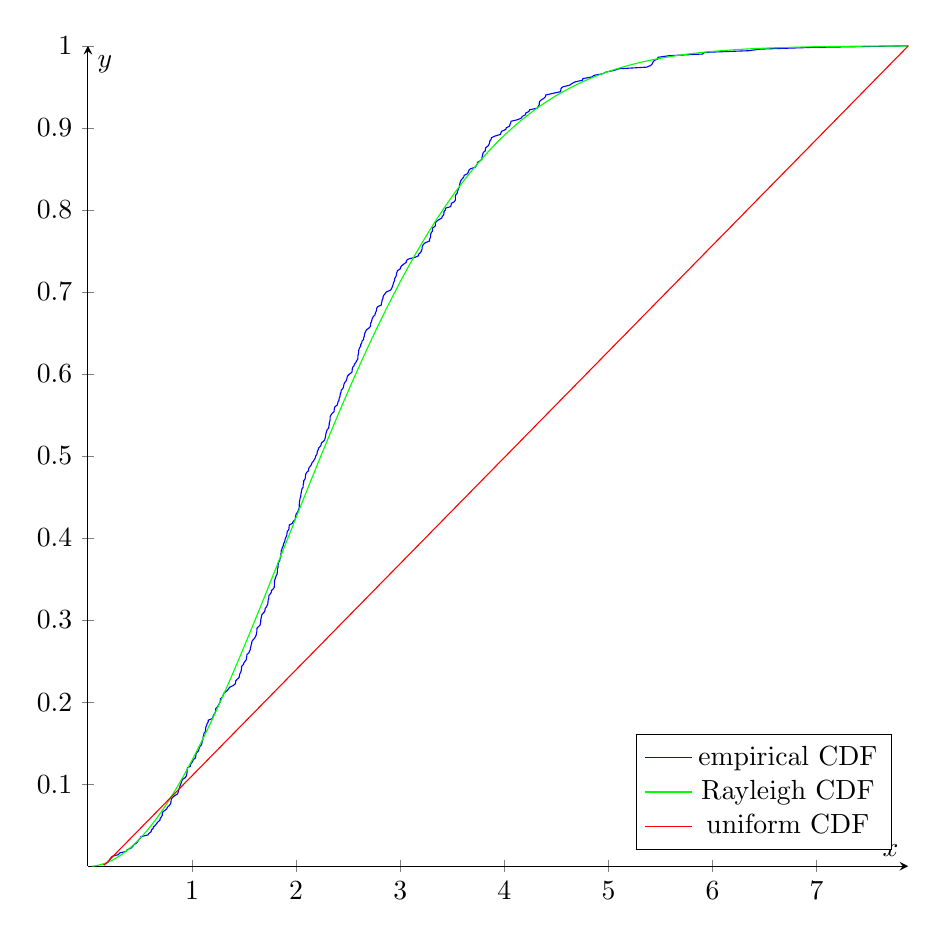
\begin{tikzpicture}
		\begin{axis}[
		xmin=0, xmax=7.8807, xlabel=$x$,
		ymin=0, ymax=1, ylabel=$y$,
		samples=401,
		axis y line=middle,
		axis x line=middle,
		restrict y to domain=0:1,
		legend style={at={(0.98,0.02)},anchor=south east},
		domain=0:7.8807,
		width=12cm,
		height=12cm,
		]
		\addplot[mark=none, blue] coordinates {
			(0.1478,0.0020)
			(0.1478,0.0020)
			(0.1832,0.0040)
			(0.1832,0.0040)
			(0.2060,0.0060)
			(0.2060,0.0060)
			(0.2075,0.0080)
			(0.2075,0.0080)
			(0.2198,0.0100)
			(0.2198,0.0100)
			(0.2329,0.0120)
			(0.2329,0.0120)
			(0.2920,0.0140)
			(0.2920,0.0140)
			(0.3034,0.0160)
			(0.3034,0.0160)
			(0.3659,0.0180)
			(0.3659,0.0180)
			(0.3767,0.0200)
			(0.3767,0.0200)
			(0.4138,0.0220)
			(0.4138,0.0220)
			(0.4305,0.0240)
			(0.4305,0.0240)
			(0.4407,0.0260)
			(0.4407,0.0260)
			(0.4646,0.0280)
			(0.4646,0.0280)
			(0.4780,0.0300)
			(0.4780,0.0300)
			(0.4862,0.0320)
			(0.4862,0.0320)
			(0.5005,0.0340)
			(0.5005,0.0340)
			(0.5102,0.0360)
			(0.5102,0.0360)
			(0.5756,0.0380)
			(0.5756,0.0380)
			(0.5863,0.0400)
			(0.5863,0.0400)
			(0.6070,0.0420)
			(0.6070,0.0420)
			(0.6099,0.0440)
			(0.6099,0.0440)
			(0.6258,0.0460)
			(0.6258,0.0460)
			(0.6314,0.0480)
			(0.6314,0.0480)
			(0.6490,0.0500)
			(0.6490,0.0500)
			(0.6595,0.0520)
			(0.6595,0.0520)
			(0.6730,0.0540)
			(0.6730,0.0540)
			(0.6918,0.0560)
			(0.6918,0.0560)
			(0.6932,0.0580)
			(0.6932,0.0580)
			(0.7054,0.0600)
			(0.7054,0.0600)
			(0.7137,0.0620)
			(0.7137,0.0620)
			(0.7138,0.0640)
			(0.7138,0.0640)
			(0.7173,0.0660)
			(0.7173,0.0660)
			(0.7403,0.0680)
			(0.7403,0.0680)
			(0.7577,0.0700)
			(0.7577,0.0700)
			(0.7640,0.0720)
			(0.7640,0.0720)
			(0.7826,0.0740)
			(0.7826,0.0740)
			(0.7935,0.0760)
			(0.7935,0.0760)
			(0.7975,0.0780)
			(0.7975,0.0780)
			(0.7990,0.0800)
			(0.7990,0.0800)
			(0.8020,0.0820)
			(0.8020,0.0820)
			(0.8155,0.0840)
			(0.8155,0.0840)
			(0.8340,0.0860)
			(0.8340,0.0860)
			(0.8603,0.0880)
			(0.8603,0.0880)
			(0.8662,0.0900)
			(0.8662,0.0900)
			(0.8707,0.0920)
			(0.8707,0.0920)
			(0.8750,0.0940)
			(0.8750,0.0940)
			(0.8808,0.0960)
			(0.8808,0.0960)
			(0.8848,0.0980)
			(0.8848,0.0980)
			(0.8914,0.1000)
			(0.8914,0.1000)
			(0.8976,0.1020)
			(0.8976,0.1020)
			(0.9016,0.1040)
			(0.9016,0.1040)
			(0.9109,0.1060)
			(0.9109,0.1060)
			(0.9358,0.1080)
			(0.9358,0.1080)
			(0.9451,0.1100)
			(0.9451,0.1100)
			(0.9494,0.1120)
			(0.9494,0.1120)
			(0.9518,0.1140)
			(0.9518,0.1140)
			(0.9519,0.1160)
			(0.9519,0.1160)
			(0.9539,0.1180)
			(0.9539,0.1180)
			(0.9560,0.1200)
			(0.9560,0.1200)
			(0.9846,0.1220)
			(0.9846,0.1220)
			(0.9847,0.1240)
			(0.9847,0.1240)
			(0.9973,0.1260)
			(0.9973,0.1260)
			(1.0050,0.1280)
			(1.0050,0.1280)
			(1.0139,0.1300)
			(1.0139,0.1300)
			(1.0324,0.1320)
			(1.0324,0.1320)
			(1.0359,0.1340)
			(1.0359,0.1340)
			(1.0361,0.1360)
			(1.0361,0.1360)
			(1.0426,0.1380)
			(1.0426,0.1380)
			(1.0590,0.1400)
			(1.0590,0.1400)
			(1.0654,0.1420)
			(1.0654,0.1420)
			(1.0684,0.1440)
			(1.0684,0.1440)
			(1.0770,0.1460)
			(1.0770,0.1460)
			(1.0911,0.1480)
			(1.0911,0.1480)
			(1.0952,0.1500)
			(1.0952,0.1500)
			(1.0952,0.1520)
			(1.0952,0.1520)
			(1.1040,0.1540)
			(1.1040,0.1540)
			(1.1057,0.1560)
			(1.1057,0.1560)
			(1.1071,0.1580)
			(1.1071,0.1580)
			(1.1126,0.1600)
			(1.1126,0.1600)
			(1.1150,0.1620)
			(1.1150,0.1620)
			(1.1282,0.1640)
			(1.1282,0.1640)
			(1.1294,0.1660)
			(1.1294,0.1660)
			(1.1300,0.1680)
			(1.1300,0.1680)
			(1.1349,0.1700)
			(1.1349,0.1700)
			(1.1410,0.1720)
			(1.1410,0.1720)
			(1.1463,0.1740)
			(1.1463,0.1740)
			(1.1560,0.1760)
			(1.1560,0.1760)
			(1.1560,0.1780)
			(1.1560,0.1780)
			(1.1956,0.1800)
			(1.1956,0.1800)
			(1.2002,0.1820)
			(1.2002,0.1820)
			(1.2068,0.1840)
			(1.2068,0.1840)
			(1.2163,0.1860)
			(1.2163,0.1860)
			(1.2249,0.1880)
			(1.2249,0.1880)
			(1.2266,0.1900)
			(1.2266,0.1900)
			(1.2276,0.1920)
			(1.2276,0.1920)
			(1.2445,0.1940)
			(1.2445,0.1940)
			(1.2513,0.1960)
			(1.2513,0.1960)
			(1.2609,0.1980)
			(1.2609,0.1980)
			(1.2706,0.2000)
			(1.2706,0.2000)
			(1.2714,0.2020)
			(1.2714,0.2020)
			(1.2728,0.2040)
			(1.2728,0.2040)
			(1.2904,0.2060)
			(1.2904,0.2060)
			(1.2985,0.2080)
			(1.2985,0.2080)
			(1.3016,0.2100)
			(1.3016,0.2100)
			(1.3159,0.2120)
			(1.3159,0.2120)
			(1.3384,0.2140)
			(1.3384,0.2140)
			(1.3516,0.2160)
			(1.3516,0.2160)
			(1.3586,0.2180)
			(1.3586,0.2180)
			(1.3927,0.2200)
			(1.3927,0.2200)
			(1.4137,0.2220)
			(1.4137,0.2220)
			(1.4186,0.2240)
			(1.4186,0.2240)
			(1.4200,0.2260)
			(1.4200,0.2260)
			(1.4348,0.2280)
			(1.4348,0.2280)
			(1.4529,0.2300)
			(1.4529,0.2300)
			(1.4543,0.2320)
			(1.4543,0.2320)
			(1.4581,0.2340)
			(1.4581,0.2340)
			(1.4663,0.2360)
			(1.4663,0.2360)
			(1.4721,0.2380)
			(1.4721,0.2380)
			(1.4741,0.2400)
			(1.4741,0.2400)
			(1.4754,0.2420)
			(1.4754,0.2420)
			(1.4782,0.2440)
			(1.4782,0.2440)
			(1.4936,0.2460)
			(1.4936,0.2460)
			(1.4992,0.2480)
			(1.4992,0.2480)
			(1.5111,0.2500)
			(1.5111,0.2500)
			(1.5224,0.2520)
			(1.5224,0.2520)
			(1.5224,0.2540)
			(1.5224,0.2540)
			(1.5265,0.2560)
			(1.5265,0.2560)
			(1.5270,0.2580)
			(1.5270,0.2580)
			(1.5467,0.2600)
			(1.5467,0.2600)
			(1.5508,0.2620)
			(1.5508,0.2620)
			(1.5605,0.2640)
			(1.5605,0.2640)
			(1.5608,0.2660)
			(1.5608,0.2660)
			(1.5661,0.2680)
			(1.5661,0.2680)
			(1.5685,0.2700)
			(1.5685,0.2700)
			(1.5736,0.2720)
			(1.5736,0.2720)
			(1.5744,0.2740)
			(1.5744,0.2740)
			(1.5871,0.2760)
			(1.5871,0.2760)
			(1.6014,0.2780)
			(1.6014,0.2780)
			(1.6099,0.2800)
			(1.6099,0.2800)
			(1.6170,0.2820)
			(1.6170,0.2820)
			(1.6185,0.2840)
			(1.6185,0.2840)
			(1.6225,0.2860)
			(1.6225,0.2860)
			(1.6233,0.2880)
			(1.6233,0.2880)
			(1.6240,0.2900)
			(1.6240,0.2900)
			(1.6389,0.2920)
			(1.6389,0.2920)
			(1.6540,0.2940)
			(1.6540,0.2940)
			(1.6569,0.2960)
			(1.6569,0.2960)
			(1.6597,0.2980)
			(1.6597,0.2980)
			(1.6600,0.3000)
			(1.6600,0.3000)
			(1.6630,0.3020)
			(1.6630,0.3020)
			(1.6667,0.3040)
			(1.6667,0.3040)
			(1.6696,0.3060)
			(1.6696,0.3060)
			(1.6796,0.3080)
			(1.6796,0.3080)
			(1.6948,0.3100)
			(1.6948,0.3100)
			(1.7011,0.3120)
			(1.7011,0.3120)
			(1.7019,0.3140)
			(1.7019,0.3140)
			(1.7140,0.3160)
			(1.7140,0.3160)
			(1.7222,0.3180)
			(1.7222,0.3180)
			(1.7280,0.3200)
			(1.7280,0.3200)
			(1.7298,0.3220)
			(1.7298,0.3220)
			(1.7306,0.3240)
			(1.7306,0.3240)
			(1.7363,0.3260)
			(1.7363,0.3260)
			(1.7380,0.3280)
			(1.7380,0.3280)
			(1.7389,0.3300)
			(1.7389,0.3300)
			(1.7525,0.3320)
			(1.7525,0.3320)
			(1.7626,0.3340)
			(1.7626,0.3340)
			(1.7628,0.3360)
			(1.7628,0.3360)
			(1.7803,0.3380)
			(1.7803,0.3380)
			(1.7892,0.3400)
			(1.7892,0.3400)
			(1.7907,0.3420)
			(1.7907,0.3420)
			(1.7907,0.3440)
			(1.7907,0.3440)
			(1.7918,0.3460)
			(1.7918,0.3460)
			(1.7926,0.3480)
			(1.7926,0.3480)
			(1.7976,0.3500)
			(1.7976,0.3500)
			(1.8039,0.3520)
			(1.8039,0.3520)
			(1.8082,0.3540)
			(1.8082,0.3540)
			(1.8170,0.3560)
			(1.8170,0.3560)
			(1.8190,0.3580)
			(1.8190,0.3580)
			(1.8193,0.3600)
			(1.8193,0.3600)
			(1.8195,0.3620)
			(1.8195,0.3620)
			(1.8254,0.3640)
			(1.8254,0.3640)
			(1.8260,0.3660)
			(1.8260,0.3660)
			(1.8276,0.3680)
			(1.8276,0.3680)
			(1.8289,0.3700)
			(1.8289,0.3700)
			(1.8420,0.3720)
			(1.8420,0.3720)
			(1.8425,0.3740)
			(1.8425,0.3740)
			(1.8497,0.3760)
			(1.8497,0.3760)
			(1.8534,0.3780)
			(1.8534,0.3780)
			(1.8535,0.3800)
			(1.8535,0.3800)
			(1.8556,0.3820)
			(1.8556,0.3820)
			(1.8557,0.3840)
			(1.8557,0.3840)
			(1.8633,0.3860)
			(1.8633,0.3860)
			(1.8654,0.3880)
			(1.8654,0.3880)
			(1.8750,0.3900)
			(1.8750,0.3900)
			(1.8771,0.3920)
			(1.8771,0.3920)
			(1.8826,0.3940)
			(1.8826,0.3940)
			(1.8905,0.3960)
			(1.8905,0.3960)
			(1.8937,0.3980)
			(1.8937,0.3980)
			(1.8975,0.4000)
			(1.8975,0.4000)
			(1.9079,0.4020)
			(1.9079,0.4020)
			(1.9111,0.4040)
			(1.9111,0.4040)
			(1.9120,0.4060)
			(1.9120,0.4060)
			(1.9151,0.4080)
			(1.9151,0.4080)
			(1.9284,0.4100)
			(1.9284,0.4100)
			(1.9315,0.4120)
			(1.9315,0.4120)
			(1.9321,0.4140)
			(1.9321,0.4140)
			(1.9351,0.4160)
			(1.9351,0.4160)
			(1.9647,0.4180)
			(1.9647,0.4180)
			(1.9702,0.4200)
			(1.9702,0.4200)
			(1.9879,0.4220)
			(1.9879,0.4220)
			(1.9936,0.4240)
			(1.9936,0.4240)
			(1.9943,0.4260)
			(1.9943,0.4260)
			(1.9972,0.4280)
			(1.9972,0.4280)
			(2.0036,0.4300)
			(2.0036,0.4300)
			(2.0165,0.4320)
			(2.0165,0.4320)
			(2.0209,0.4340)
			(2.0209,0.4340)
			(2.0281,0.4360)
			(2.0281,0.4360)
			(2.0295,0.4380)
			(2.0295,0.4380)
			(2.0299,0.4400)
			(2.0299,0.4400)
			(2.0306,0.4420)
			(2.0306,0.4420)
			(2.0319,0.4440)
			(2.0319,0.4440)
			(2.0352,0.4460)
			(2.0352,0.4460)
			(2.0364,0.4480)
			(2.0364,0.4480)
			(2.0435,0.4500)
			(2.0435,0.4500)
			(2.0448,0.4520)
			(2.0448,0.4520)
			(2.0466,0.4540)
			(2.0466,0.4540)
			(2.0504,0.4560)
			(2.0504,0.4560)
			(2.0528,0.4580)
			(2.0528,0.4580)
			(2.0563,0.4600)
			(2.0563,0.4600)
			(2.0669,0.4620)
			(2.0669,0.4620)
			(2.0674,0.4640)
			(2.0674,0.4640)
			(2.0694,0.4660)
			(2.0694,0.4660)
			(2.0733,0.4680)
			(2.0733,0.4680)
			(2.0735,0.4700)
			(2.0735,0.4700)
			(2.0862,0.4720)
			(2.0862,0.4720)
			(2.0884,0.4740)
			(2.0884,0.4740)
			(2.0905,0.4760)
			(2.0905,0.4760)
			(2.0924,0.4780)
			(2.0924,0.4780)
			(2.1019,0.4800)
			(2.1019,0.4800)
			(2.1187,0.4820)
			(2.1187,0.4820)
			(2.1198,0.4840)
			(2.1198,0.4840)
			(2.1257,0.4860)
			(2.1257,0.4860)
			(2.1386,0.4880)
			(2.1386,0.4880)
			(2.1486,0.4900)
			(2.1486,0.4900)
			(2.1533,0.4920)
			(2.1533,0.4920)
			(2.1679,0.4940)
			(2.1679,0.4940)
			(2.1765,0.4960)
			(2.1765,0.4960)
			(2.1849,0.4980)
			(2.1849,0.4980)
			(2.1883,0.5000)
			(2.1883,0.5000)
			(2.1991,0.5020)
			(2.1991,0.5020)
			(2.2022,0.5040)
			(2.2022,0.5040)
			(2.2035,0.5060)
			(2.2035,0.5060)
			(2.2138,0.5080)
			(2.2138,0.5080)
			(2.2173,0.5100)
			(2.2173,0.5100)
			(2.2343,0.5120)
			(2.2343,0.5120)
			(2.2400,0.5140)
			(2.2400,0.5140)
			(2.2436,0.5160)
			(2.2436,0.5160)
			(2.2638,0.5180)
			(2.2638,0.5180)
			(2.2755,0.5200)
			(2.2755,0.5200)
			(2.2784,0.5220)
			(2.2784,0.5220)
			(2.2830,0.5240)
			(2.2830,0.5240)
			(2.2843,0.5260)
			(2.2843,0.5260)
			(2.2879,0.5280)
			(2.2879,0.5280)
			(2.2925,0.5300)
			(2.2925,0.5300)
			(2.2984,0.5320)
			(2.2984,0.5320)
			(2.3128,0.5340)
			(2.3128,0.5340)
			(2.3139,0.5360)
			(2.3139,0.5360)
			(2.3175,0.5380)
			(2.3175,0.5380)
			(2.3183,0.5400)
			(2.3183,0.5400)
			(2.3234,0.5420)
			(2.3234,0.5420)
			(2.3259,0.5440)
			(2.3259,0.5440)
			(2.3259,0.5460)
			(2.3259,0.5460)
			(2.3260,0.5480)
			(2.3260,0.5480)
			(2.3351,0.5500)
			(2.3351,0.5500)
			(2.3456,0.5520)
			(2.3456,0.5520)
			(2.3648,0.5540)
			(2.3648,0.5540)
			(2.3654,0.5560)
			(2.3654,0.5560)
			(2.3672,0.5580)
			(2.3672,0.5580)
			(2.3730,0.5600)
			(2.3730,0.5600)
			(2.3940,0.5620)
			(2.3940,0.5620)
			(2.3997,0.5640)
			(2.3997,0.5640)
			(2.4025,0.5660)
			(2.4025,0.5660)
			(2.4116,0.5680)
			(2.4116,0.5680)
			(2.4126,0.5700)
			(2.4126,0.5700)
			(2.4204,0.5720)
			(2.4204,0.5720)
			(2.4224,0.5740)
			(2.4224,0.5740)
			(2.4248,0.5760)
			(2.4248,0.5760)
			(2.4314,0.5780)
			(2.4314,0.5780)
			(2.4323,0.5800)
			(2.4323,0.5800)
			(2.4466,0.5820)
			(2.4466,0.5820)
			(2.4557,0.5840)
			(2.4557,0.5840)
			(2.4571,0.5860)
			(2.4571,0.5860)
			(2.4604,0.5880)
			(2.4604,0.5880)
			(2.4704,0.5900)
			(2.4704,0.5900)
			(2.4822,0.5920)
			(2.4822,0.5920)
			(2.4873,0.5940)
			(2.4873,0.5940)
			(2.4896,0.5960)
			(2.4896,0.5960)
			(2.4970,0.5980)
			(2.4970,0.5980)
			(2.5136,0.6000)
			(2.5136,0.6000)
			(2.5357,0.6020)
			(2.5357,0.6020)
			(2.5379,0.6040)
			(2.5379,0.6040)
			(2.5392,0.6060)
			(2.5392,0.6060)
			(2.5431,0.6080)
			(2.5431,0.6080)
			(2.5558,0.6100)
			(2.5558,0.6100)
			(2.5603,0.6120)
			(2.5603,0.6120)
			(2.5738,0.6140)
			(2.5738,0.6140)
			(2.5808,0.6160)
			(2.5808,0.6160)
			(2.5915,0.6180)
			(2.5915,0.6180)
			(2.5934,0.6200)
			(2.5934,0.6200)
			(2.5937,0.6220)
			(2.5937,0.6220)
			(2.5965,0.6240)
			(2.5965,0.6240)
			(2.5999,0.6260)
			(2.5999,0.6260)
			(2.6005,0.6280)
			(2.6005,0.6280)
			(2.6036,0.6300)
			(2.6036,0.6300)
			(2.6100,0.6320)
			(2.6100,0.6320)
			(2.6203,0.6340)
			(2.6203,0.6340)
			(2.6210,0.6360)
			(2.6210,0.6360)
			(2.6307,0.6380)
			(2.6307,0.6380)
			(2.6325,0.6400)
			(2.6325,0.6400)
			(2.6473,0.6420)
			(2.6473,0.6420)
			(2.6486,0.6440)
			(2.6486,0.6440)
			(2.6546,0.6460)
			(2.6546,0.6460)
			(2.6556,0.6480)
			(2.6556,0.6480)
			(2.6613,0.6500)
			(2.6613,0.6500)
			(2.6683,0.6520)
			(2.6683,0.6520)
			(2.6768,0.6540)
			(2.6768,0.6540)
			(2.7001,0.6560)
			(2.7001,0.6560)
			(2.7133,0.6580)
			(2.7133,0.6580)
			(2.7151,0.6600)
			(2.7151,0.6600)
			(2.7159,0.6620)
			(2.7159,0.6620)
			(2.7251,0.6640)
			(2.7251,0.6640)
			(2.7273,0.6660)
			(2.7273,0.6660)
			(2.7330,0.6680)
			(2.7330,0.6680)
			(2.7413,0.6700)
			(2.7413,0.6700)
			(2.7579,0.6720)
			(2.7579,0.6720)
			(2.7603,0.6740)
			(2.7603,0.6740)
			(2.7677,0.6760)
			(2.7677,0.6760)
			(2.7732,0.6780)
			(2.7732,0.6780)
			(2.7735,0.6800)
			(2.7735,0.6800)
			(2.7834,0.6820)
			(2.7834,0.6820)
			(2.8180,0.6840)
			(2.8180,0.6840)
			(2.8190,0.6860)
			(2.8190,0.6860)
			(2.8236,0.6880)
			(2.8236,0.6880)
			(2.8258,0.6900)
			(2.8258,0.6900)
			(2.8339,0.6920)
			(2.8339,0.6920)
			(2.8349,0.6940)
			(2.8349,0.6940)
			(2.8426,0.6960)
			(2.8426,0.6960)
			(2.8548,0.6980)
			(2.8548,0.6980)
			(2.8668,0.7000)
			(2.8668,0.7000)
			(2.9042,0.7020)
			(2.9042,0.7020)
			(2.9168,0.7040)
			(2.9168,0.7040)
			(2.9232,0.7060)
			(2.9232,0.7060)
			(2.9294,0.7080)
			(2.9294,0.7080)
			(2.9334,0.7100)
			(2.9334,0.7100)
			(2.9382,0.7120)
			(2.9382,0.7120)
			(2.9453,0.7140)
			(2.9453,0.7140)
			(2.9460,0.7160)
			(2.9460,0.7160)
			(2.9543,0.7180)
			(2.9543,0.7180)
			(2.9630,0.7200)
			(2.9630,0.7200)
			(2.9636,0.7220)
			(2.9636,0.7220)
			(2.9680,0.7240)
			(2.9680,0.7240)
			(2.9753,0.7260)
			(2.9753,0.7260)
			(2.9996,0.7280)
			(2.9996,0.7280)
			(3.0034,0.7300)
			(3.0034,0.7300)
			(3.0149,0.7320)
			(3.0149,0.7320)
			(3.0348,0.7340)
			(3.0348,0.7340)
			(3.0571,0.7360)
			(3.0571,0.7360)
			(3.0592,0.7380)
			(3.0592,0.7380)
			(3.0761,0.7400)
			(3.0761,0.7400)
			(3.1380,0.7420)
			(3.1380,0.7420)
			(3.1749,0.7440)
			(3.1749,0.7440)
			(3.1777,0.7460)
			(3.1777,0.7460)
			(3.1949,0.7480)
			(3.1949,0.7480)
			(3.2042,0.7500)
			(3.2042,0.7500)
			(3.2098,0.7520)
			(3.2098,0.7520)
			(3.2105,0.7540)
			(3.2105,0.7540)
			(3.2141,0.7560)
			(3.2141,0.7560)
			(3.2232,0.7580)
			(3.2232,0.7580)
			(3.2414,0.7600)
			(3.2414,0.7600)
			(3.2813,0.7620)
			(3.2813,0.7620)
			(3.2814,0.7640)
			(3.2814,0.7640)
			(3.2887,0.7660)
			(3.2887,0.7660)
			(3.2923,0.7680)
			(3.2923,0.7680)
			(3.2924,0.7700)
			(3.2924,0.7700)
			(3.2967,0.7720)
			(3.2967,0.7720)
			(3.3087,0.7740)
			(3.3087,0.7740)
			(3.3105,0.7760)
			(3.3105,0.7760)
			(3.3115,0.7780)
			(3.3115,0.7780)
			(3.3351,0.7800)
			(3.3351,0.7800)
			(3.3371,0.7820)
			(3.3371,0.7820)
			(3.3372,0.7840)
			(3.3372,0.7840)
			(3.3482,0.7860)
			(3.3482,0.7860)
			(3.3707,0.7880)
			(3.3707,0.7880)
			(3.3981,0.7900)
			(3.3981,0.7900)
			(3.4042,0.7920)
			(3.4042,0.7920)
			(3.4174,0.7940)
			(3.4174,0.7940)
			(3.4200,0.7960)
			(3.4200,0.7960)
			(3.4205,0.7980)
			(3.4205,0.7980)
			(3.4339,0.8000)
			(3.4339,0.8000)
			(3.4340,0.8020)
			(3.4340,0.8020)
			(3.4838,0.8040)
			(3.4838,0.8040)
			(3.4891,0.8060)
			(3.4891,0.8060)
			(3.4915,0.8080)
			(3.4915,0.8080)
			(3.5200,0.8100)
			(3.5200,0.8100)
			(3.5293,0.8120)
			(3.5293,0.8120)
			(3.5300,0.8140)
			(3.5300,0.8140)
			(3.5303,0.8160)
			(3.5303,0.8160)
			(3.5310,0.8180)
			(3.5310,0.8180)
			(3.5465,0.8200)
			(3.5465,0.8200)
			(3.5486,0.8220)
			(3.5486,0.8220)
			(3.5550,0.8240)
			(3.5550,0.8240)
			(3.5595,0.8260)
			(3.5595,0.8260)
			(3.5684,0.8280)
			(3.5684,0.8280)
			(3.5694,0.8300)
			(3.5694,0.8300)
			(3.5730,0.8320)
			(3.5730,0.8320)
			(3.5775,0.8340)
			(3.5775,0.8340)
			(3.5835,0.8360)
			(3.5835,0.8360)
			(3.5968,0.8380)
			(3.5968,0.8380)
			(3.6101,0.8400)
			(3.6101,0.8400)
			(3.6133,0.8420)
			(3.6133,0.8420)
			(3.6449,0.8440)
			(3.6449,0.8440)
			(3.6529,0.8460)
			(3.6529,0.8460)
			(3.6582,0.8480)
			(3.6582,0.8480)
			(3.6729,0.8500)
			(3.6729,0.8500)
			(3.7202,0.8520)
			(3.7202,0.8520)
			(3.7309,0.8540)
			(3.7309,0.8540)
			(3.7402,0.8560)
			(3.7402,0.8560)
			(3.7421,0.8580)
			(3.7421,0.8580)
			(3.7704,0.8600)
			(3.7704,0.8600)
			(3.7853,0.8620)
			(3.7853,0.8620)
			(3.7854,0.8640)
			(3.7854,0.8640)
			(3.7904,0.8660)
			(3.7904,0.8660)
			(3.7930,0.8680)
			(3.7930,0.8680)
			(3.7976,0.8700)
			(3.7976,0.8700)
			(3.8171,0.8720)
			(3.8171,0.8720)
			(3.8175,0.8740)
			(3.8175,0.8740)
			(3.8229,0.8760)
			(3.8229,0.8760)
			(3.8442,0.8780)
			(3.8442,0.8780)
			(3.8531,0.8800)
			(3.8531,0.8800)
			(3.8585,0.8820)
			(3.8585,0.8820)
			(3.8606,0.8840)
			(3.8606,0.8840)
			(3.8726,0.8860)
			(3.8726,0.8860)
			(3.8772,0.8880)
			(3.8772,0.8880)
			(3.9105,0.8900)
			(3.9105,0.8900)
			(3.9622,0.8920)
			(3.9622,0.8920)
			(3.9671,0.8940)
			(3.9671,0.8940)
			(3.9767,0.8960)
			(3.9767,0.8960)
			(4.0148,0.8980)
			(4.0148,0.8980)
			(4.0175,0.9000)
			(4.0175,0.9000)
			(4.0500,0.9020)
			(4.0500,0.9020)
			(4.0532,0.9040)
			(4.0532,0.9040)
			(4.0618,0.9060)
			(4.0618,0.9060)
			(4.0636,0.9080)
			(4.0636,0.9080)
			(4.1300,0.9100)
			(4.1300,0.9100)
			(4.1635,0.9120)
			(4.1635,0.9120)
			(4.1724,0.9140)
			(4.1724,0.9140)
			(4.2040,0.9160)
			(4.2040,0.9160)
			(4.2042,0.9180)
			(4.2042,0.9180)
			(4.2367,0.9200)
			(4.2367,0.9200)
			(4.2417,0.9220)
			(4.2417,0.9220)
			(4.3178,0.9240)
			(4.3178,0.9240)
			(4.3248,0.9260)
			(4.3248,0.9260)
			(4.3350,0.9280)
			(4.3350,0.9280)
			(4.3354,0.9300)
			(4.3354,0.9300)
			(4.3376,0.9320)
			(4.3376,0.9320)
			(4.3542,0.9340)
			(4.3542,0.9340)
			(4.3792,0.9360)
			(4.3792,0.9360)
			(4.3957,0.9380)
			(4.3957,0.9380)
			(4.3975,0.9400)
			(4.3975,0.9400)
			(4.4643,0.9420)
			(4.4643,0.9420)
			(4.5387,0.9440)
			(4.5387,0.9440)
			(4.5428,0.9460)
			(4.5428,0.9460)
			(4.5447,0.9480)
			(4.5447,0.9480)
			(4.5609,0.9500)
			(4.5609,0.9500)
			(4.6277,0.9520)
			(4.6277,0.9520)
			(4.6497,0.9540)
			(4.6497,0.9540)
			(4.6792,0.9560)
			(4.6792,0.9560)
			(4.7490,0.9580)
			(4.7490,0.9580)
			(4.7546,0.9600)
			(4.7546,0.9600)
			(4.8401,0.9620)
			(4.8401,0.9620)
			(4.8610,0.9640)
			(4.8610,0.9640)
			(4.9467,0.9660)
			(4.9467,0.9660)
			(4.9772,0.9680)
			(4.9772,0.9680)
			(5.0550,0.9700)
			(5.0550,0.9700)
			(5.0998,0.9720)
			(5.0998,0.9720)
			(5.3684,0.9740)
			(5.3684,0.9740)
			(5.4054,0.9760)
			(5.4054,0.9760)
			(5.4206,0.9780)
			(5.4206,0.9780)
			(5.4268,0.9800)
			(5.4268,0.9800)
			(5.4398,0.9820)
			(5.4398,0.9820)
			(5.4733,0.9840)
			(5.4733,0.9840)
			(5.4752,0.9860)
			(5.4752,0.9860)
			(5.5878,0.9880)
			(5.5878,0.9880)
			(5.9050,0.9900)
			(5.9050,0.9900)
			(5.9230,0.9920)
			(5.9230,0.9920)
			(6.3455,0.9940)
			(6.3455,0.9940)
			(6.4626,0.9960)
			(6.4626,0.9960)
			(6.9462,0.9980)
			(6.9462,0.9980)
			(7.8807,1.0000)
			(7.8807,1.0000)
		};
		\addlegendentry{empirical CDF};
		\addplot[mark=none,green] {1-exp(-x^2/(2*3.6111))};
		\addlegendentry{\person{Rayleigh} CDF};
		\addplot[mark=none,red] {(x-0.1478)/7.7329};
		\addlegendentry{uniform CDF};
		\end{axis}
		\end{tikzpicture}
\end{center}

\pagebreak
\section{Task 4}
\subsection{Part (1)}
The probability density function $f(t)$ is
\begin{align}
	f(t) = \frac{2t\cdot\frac{\exp(-t^2)}{100}}{100} = \frac{t\cdot\exp(-t^2)}{5000}\notag
\end{align}
\begin{center}
	\begin{tikzpicture}
	\begin{axis}[
	xmin=0, xmax=5, xlabel=$x$,
	ymin=0, ymax=0.0001, ylabel=$y$,
	samples=400,
	axis y line=middle,
	axis x line=middle,
	restrict y to domain=0:1,
	]
	\addplot+[mark=none] {(x*exp(-x^2))/5000};
	\end{axis}
	\end{tikzpicture}
\end{center}
The cumulative distribution function $F(t)$ is then
\begin{align}
	F(t) &= \int_0^t f(\xi)\,\diff\xi \notag \\
	&= \int_0^t \frac{\xi\cdot\exp(-\xi^2)}{5000}\,\diff\xi\notag \\
	&= \frac{\exp(-t^2)\Big(\exp(t^2)-1\Big)}{10000} \notag
\end{align}
\begin{center}
	\begin{tikzpicture}
	\begin{axis}[
	xmin=0, xmax=5, xlabel=$x$,
	ymin=0, ymax=0.0001, ylabel=$y$,
	samples=400,
	axis y line=middle,
	axis x line=middle,
	restrict y to domain=0:1,
	]
	\addplot+[mark=none] {(exp(-x^2)*(exp(x^2)-1))/10000};
	\end{axis}
	\end{tikzpicture}
\end{center}
For the survival function we get
\begin{align}
	R(t) &= 1 - F(t) \notag \\
	&= \frac{\exp(-t^2)+9999}{10000} \notag
\end{align}
\begin{center}
	\begin{tikzpicture}[scale=0.9]
	\begin{axis}[
	xmin=0, xmax=5, xlabel=$x$,
	ymin=0, ymax=1, ylabel=$y$,
	samples=400,
	axis y line=middle,
	axis x line=middle,
	restrict y to domain=0:1,
	]
	\addplot+[mark=none] {(exp(-x^2)+9999)/10000};
	\end{axis}
	\end{tikzpicture}
	\begin{tikzpicture}[scale=0.9]
	\begin{axis}[
	xmin=0, xmax=5, xlabel=$x$,
	ymin=0.9999, ymax=1, ylabel=$y$,
	samples=400,
	axis y line=middle,
	axis x line=middle,
	restrict y to domain=0:1,
	y tick label style={
		/pgf/number format/.cd,
		precision=5,
		/tikz/.cd
	},
	]
	\addplot+[mark=none] {(exp(-x^2)+9999)/10000};
	\end{axis}
	\end{tikzpicture}
\end{center}
To get the reliability of the component at $t=7$ we simply evaluate $R(7)$ which is 0.9999.

The hazard function is defined as
\begin{align}
	h(t) &= \frac{f(t)}{1-F(t)} \notag \\
	&= \frac{2t}{9999\cdot \exp(t^2)+1} \notag
\end{align}
\begin{center}
	\begin{tikzpicture}
	\begin{axis}[
	xmin=0, xmax=5, xlabel=$x$,
	ymin=0, ymax=0.0001, ylabel=$y$,
	samples=400,
	axis y line=middle,
	axis x line=middle,
	restrict y to domain=0:1,
	]
	\addplot+[mark=none] {(2*x)/(9999*exp(x^2)+1)};
	\end{axis}
	\end{tikzpicture}
\end{center}
The hazard function describes how an item ages where $t$ affects the risk of failure. It is the frequency with which the item fails, expressed in failures per unit of time.

\subsection{Part (2)}
Given $h(x)\sim(\sqrt{x})^{-1}$ we will try to find out the $shape$-parameter of the \person{Weibull} distribution first.
\begin{center}
	\begin{tikzpicture}
	\begin{axis}[
	xmin=0, xmax=5, xlabel=$x$,
	ymin=0, ymax=1, ylabel=$y$,
	samples=400,
	axis y line=middle,
	axis x line=middle,
	restrict y to domain=0:1,
	yticklabels={,,},
	xticklabels={,,}
	]
	\addplot+[mark=none] {1/sqrt(x)};
	\end{axis}
	\end{tikzpicture}
\end{center}
Comparing this graph to graphs of the hazard function with different $shape$-parameters we see that $shape=0.5$ fits best.
\begin{center}
	\begin{tabular}{p{5cm}|p{5cm}|p{5cm}}
		$shape = 0.5$ & $shape = 1$ & $shape = 2$ \\
		\hline
		\multicolumn{3}{c}{\cellcolor{gray!50}\textbf{Hazard function} $\left(h = \frac{\text{PDF}}{1-\text{CDF}}\right)$} \\
		\hline
		\begin{tikzpicture}[scale=0.6]
		\begin{axis}[
		xmin=0, xmax=2, xlabel=$x$,
		ymin=0, ymax=1, ylabel=$y$,
		samples=400,
		axis y line=middle,
		axis x line=middle,
		]
		\addplot+[mark=none] {(0.5*x^(-0.5)*exp(-x^0.5))/(1-(1-exp(-x^0.5)))};
		\end{axis}
		\end{tikzpicture} &
		\begin{tikzpicture}[scale=0.6]
		\begin{axis}[
		xmin=0, xmax=2, xlabel=$x$,
		ymin=0, ymax=1, ylabel=$y$,
		samples=400,
		axis y line=middle,
		axis x line=middle,
		restrict y to domain=0:1,
		]
		\addplot+[mark=none] {(1/exp(x))/(1-(1-1/exp(x)))};
		\draw[blue] (axis cs: 0,1) -- (axis cs: 2,1);
		\end{axis}
		\end{tikzpicture} &
		\begin{tikzpicture}[scale=0.6]
		\begin{axis}[
		xmin=0, xmax=2, xlabel=$x$,
		ymin=0, ymax=1, ylabel=$y$,
		samples=400,
		axis y line=middle,
		axis x line=middle,
		]
		\addplot+[mark=none] {(2*x^(1)*exp(-x^2))/(1-(1-exp(-x^2)))};
		\end{axis}
		\end{tikzpicture} \\
	    \end{tabular}
\end{center}
To get the $scale$-parameter of the distribution we use the other provided information:
\begin{align}
	5 &= \mu \notag \\
	&= scale\cdot\Gamma\left(1+\frac{1}{shape}\right) \notag \\
	&= scale\cdot\Gamma(3) \notag \\
	\Rightarrow scale &= \frac{5}{2} \notag
\end{align}
Let's build the survival function:
\begin{align}
	R(t) &= 1-\Bigg(1-\exp\left(-\sqrt{\frac{x}{\nicefrac{5}{2}}}\right)\Bigg) \notag \\
	&= \exp(-\sqrt{x}\cdot\sqrt{2.5})\notag
\end{align}
That mean that the probability of surviving 6 years (30 years) is $R(6) = 0.0208$ ($R(30) = 0.0002$).
\end{document}
